\section{Appendix}
\label{sec:mpt}

%This is not a correct appendix page
\begin{enumerate}
    \item Editable figma files: \\
    \url{https://www.figma.com/file/QHZrqRKHQ3I0fOFJN3Fcwu/DevOps2022?node-id=0\%3A1}
    \item Security Assessment: \\
    \url{https://github.com/Faurby/BlackOps/blob/main/Security_Assessment.md}
    \item Github Repository Workflows: \\    \url{https://github.com/Faurby/BlackOps/tree/main/.github/workflows}
    \item GitHub Repository Pull-Request:\\
    \url{https://github.com/Faurby/BlackOps/pull/63}
    \begin{figure}[H]
    \centering
    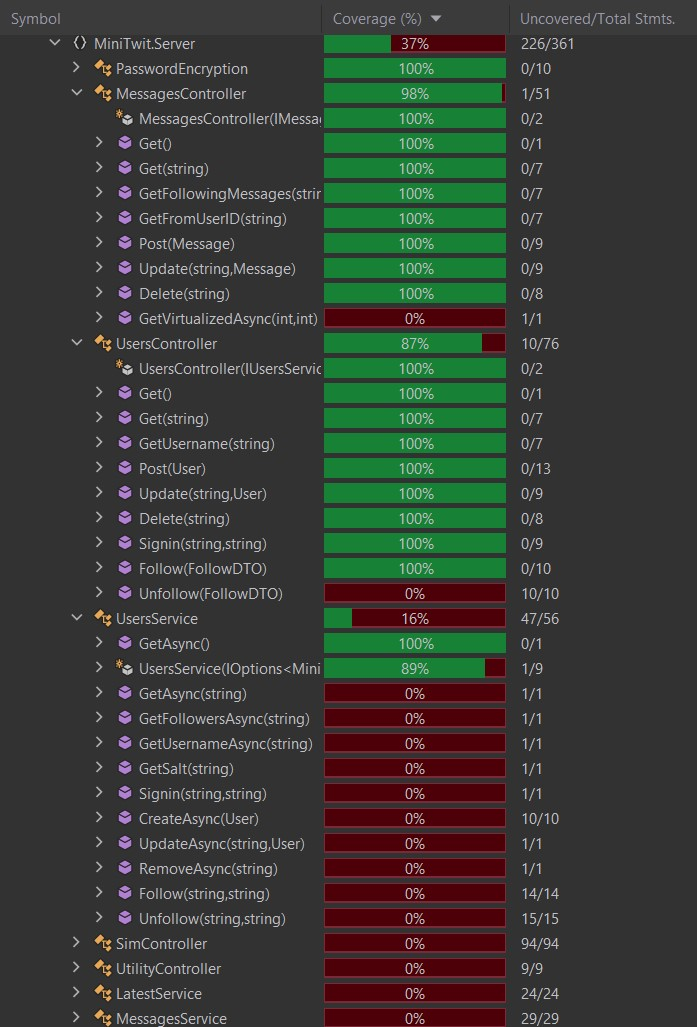
\includegraphics[width=16cm,height=14cm,keepaspectratio]{Diagrams/test coverage server.jpg}
    \caption{Test coverage of the server assembly.}
    \label{ServerAssembly}
    \end{figure}
    \item \textit{System dependencies:}\\\\
    \textit{Docker images:}
    \begin{itemize}
        \item Docker@20.10.16
        \item Docker-Compose@1.25.0
    
        \item Grafana@8.4.0
        \item Prometheus@latest
        
        \item FileBeat@7.17.1
        \item ElasticSearch@7.17.1
        \item Kibana@7.17.1
        \item nginx@latest
        
        \item dotnet/sdk@6.0
        \item MongoDB@5.0
        \item Ubuntu@20.04
    \end{itemize}
    \textbf{MiniTwit C\# Application}:\\\\
    \textit{Server:}
    \begin{itemize}
        \item BCrypt.Net-Next@4.0.2
        \item Blazored.LocalStorage@4.2.0
        \item Blazored.Modal@6.0.1
        \item Microsoft.AspNetCore.Components.WebAssembly.Server@6.0.1
        \item Mongo2Go@3.1.3
        \item MongoDB.Driver@2.14.1
        \item prometheus-net.AspNetCore@6.0.0
        \item Swashbuckle.AspNetCore@6.2.3
    \end{itemize}
    \textit{Server.Tests}
    \begin{itemize}
        \item coverlet.collector@3.1.0
        \item Microsoft.Extensions.Options@6.0.0
        \item Microsoft.Net.Test.Sdk@16.11.0
        \item Mongo2Go@3.1.3
        \item MongoDB.Driver@2.24.1
        \item Moq@4.16.1
        \item xunit@2.4.1
        \item xunit.runner.visualstudio@2.4.3
    \end{itemize}
    \textit{Client}
    \begin{itemize}
        \item Blazored.LocalStorage@4.2.0
        \item Blazored.Modal@6.0.1
        \item Microsoft.AspNetCore.Components.WebAssembly@6.0.1
    \end{itemize}
    \textit{Shared}
    \begin{itemize}
        \item MongoDB.Driver@2.14.1
    \end{itemize}
    \textbf{CI / CD Tools}\\\\
    \textit{Deploy}
    \begin{itemize}
         \item actions/checkout@v2
         \item docker/login-action@v1
         \item fifsky/ssh-action@master
         \item Vagrant@2.2.19
    \end{itemize}
      
    \textit{Build and test}
    \begin{itemize}
         \item actions/setup-dotnet@v1
    \end{itemize}
    
    \textit{Release maker}
    \begin{itemize}
         \item WyriHaximus/github-action-next-semvers@v1
         \item actions/create-release@v1
         \item metcalfc/changelog-generator@v3.0.0
    \end{itemize}
    
    \textit{Snyk scanning}
    \begin{itemize}
         \item snyk/actions/docker@master
         \item github/codeql-action/upload-sarif@v1
    \end{itemize}
    
    \textit{SonarCloud}
    \begin{itemize}
        \item actions/setup-java@v1
        \item actions/cache@v1
        \item sonarscanner@latest
    \end{itemize}
    
    \textit{Yaml lint}
    \begin{itemize}
        \item yamllint@latest
    \end{itemize}
    \item First Database Crash 

    29-03-2022

    What happened and how
    \begin{itemize}
        \item Tried to implement logging
        \item Volumesdidn’t work leading to data getting lost when trying to revert
        \item Database then crashed when trying to regain the lost data
    \end{itemize}
   
    Result:
    \begin{itemize}
        \item Database was lost
        \item Last backup was 1 week old
        \item Lots of missing users in backup leading to tweet, follow and unfollow errors where users did not exist
        \item Panic
    \end{itemize}
    
    
    Reflections:
    \begin{itemize}
        \item Docker Swarm considerations
        \begin{itemize}
            \item Assumption is that droplets do not crash, more likely our service crashes. Therefore everything is docker containers on the same droplet
        \end{itemize}
        \item Solutions
        \begin{itemize}
            \item Fix volumes
            \item Create workflow that backups database regularly (cron job maybe once a day?)
            \item move database to own droplet
        \end{itemize}
    \end{itemize}
    
    \item Second Database Crash
    
    04-04-2022

    What happened and how:
    \begin{itemize}
        \item New update to main got pushed
        \item Tried to update logging
        \item Docker compose up started logging, which used a lot of memory and slowed everything down
        \item Tried to docker compose down to close containers and ensure that droplets did not die
        \item Docker compose down cleared out our containers, and thereby our volumes and all our data
        \item Tried Docker compose up again after, where docker tried to pull from the now empty volume
    \end{itemize}
    
    Result:
    \begin{itemize}
        \item Database was lost
        \item Last backup was 2 weeks old
        \item New batch had just started
        \item Lots of missing users in backup leading to tweet, follow and unfollow errors where users did not exist
        \item More panic
    \end{itemize}
    
    Reflections:
    \begin{itemize}
        \item Docker swarm considerations
        \begin{itemize}
            \item More considerations done regarding the amount of manager and worker nodes needed
            \item More considerations done regarding where (and how) to use logging and monitoring
            \item Started working on docker swarms
        \end{itemize}
        \item Solutions
        \begin{itemize}
            \item Volumes got pushed right after
            \item Create workflow that backups database regularly (cron job maybe once a day?). Starting to sound like a good idea
            \item Considerations done regarding moving the database into separate droplet
        \end{itemize}
    \end{itemize}
\end{enumerate}
